\section{Computer Vision}
Computer Vision is a field of Artificial Intelligence and Computer Science that aims at giving computers a visual understanding of the world.

The goal of Computer Vision is to emulate human vision using digital images through three main processing components, executed one after the other:
\begin{itemize}
    \item Image acquisition.
    \item Image processing.
    \item Image analysis and understanding.
\end{itemize}
\begin{figure}[H]
\centering
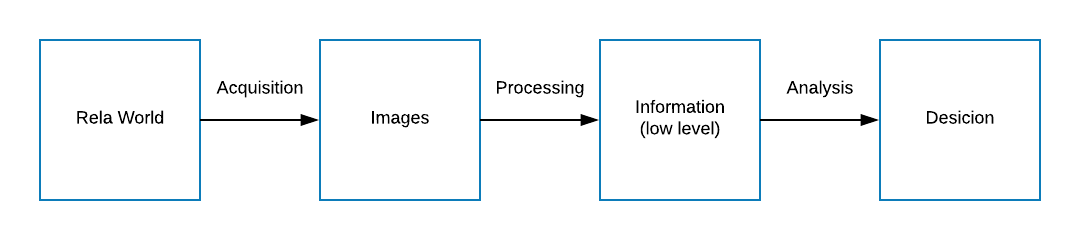
\includegraphics[width=10cm,height=10cm,keepaspectratio]{imagenes/ComputerVisionBlocks.png}
\caption{Computer Vision work flow}
\label{fig:ComputerVision}
\end{figure}
As the human visual understanding of the world is reflected in the ability to make decisions through what humans see, providing such a visual understanding to computers would allow them the same capabilities.

\subsection{Image acquisition}
Image acquisition is the process of translating the analog data into binary data. Interpreted as digital images.
Different tools have been created to build such datasets:
\begin{itemize}
    \item Webcams and embedded cameras.
    \item Digital compact cameras and DSLR.
    \item Consumer 3D cameras and laser rangefinders.
\end{itemize}
Most of the time, the raw data acquired by these devices need to be post-processed to be more efficiently exploited in the next steps.

\subsection{Image processing}
The second component of Computer Vision is the low-level processing of images. Algorithms are applied to the binary data acquired in the first step to infer low-level information on parts of the image. This type of information is characterized by image edges, point features or segments, for example.

This second step usually involves advanced applied mathematics algorithms and techniques.

Low-level image processing algorithms include:
\begin{itemize}
    \item Edge detection.
    \item Segmentation.
    \item Classification.
    \item Feature detection and matching.
\end{itemize}

\subsection{Image analysis and understanding}
The last step of the Computer Vision pipeline is the actual analysis of the data, which allow the decision making.
High-level algorithms are applied, using both the image data and the low-level information computed in previous steps.

Examples of high-level image analysis are:
\begin{itemize}
    \item 3D scene mapping.
    \item Object recognition.
    \item Object tracking.
\end{itemize}
\subsection{Applications of computer vision}
Techniques developed for computer vision have many application in the fields of robotics, human-computer interaction and visualization, to name a few.
\begin{enumerate}
    \item Motion recognition.
    \item Augmented reality.
    \item Autonomous cars.
    \item Domestic robots.
    \item Image restoration.
\end{enumerate}

\subsection{JeVois Camera}
JeVois is a small, open-source, smart machine vision camera that was funded on Kickstarter in early 2017. It runs embedded Linux and can process video at high frame rates using OpenCV algorithms. It can run standalone, or as a USB camera, streaming raw or pre-processed video to a host computer for further action. In either case, it can communicate to (and be controlled by) other devices via the serial port.

The JeVois framework operates as follows: video is captured from the camera sensor, processed on the fly through some machine vision algorithm directly on the camera's processor, and the results are streamed over USB to a host computer and/or over serial to a micro-controller.

To the host computer, the JeVois smart camera is just another USB camera. Different vision algorithms are selected by changing USB camera resolution and framerate. Users or machines can also interact with the JeVois smart camera, change its settings, or listen for text-based vision outputs over serial link.\cite{JeVois}
\begin{figure}[H]
\centering
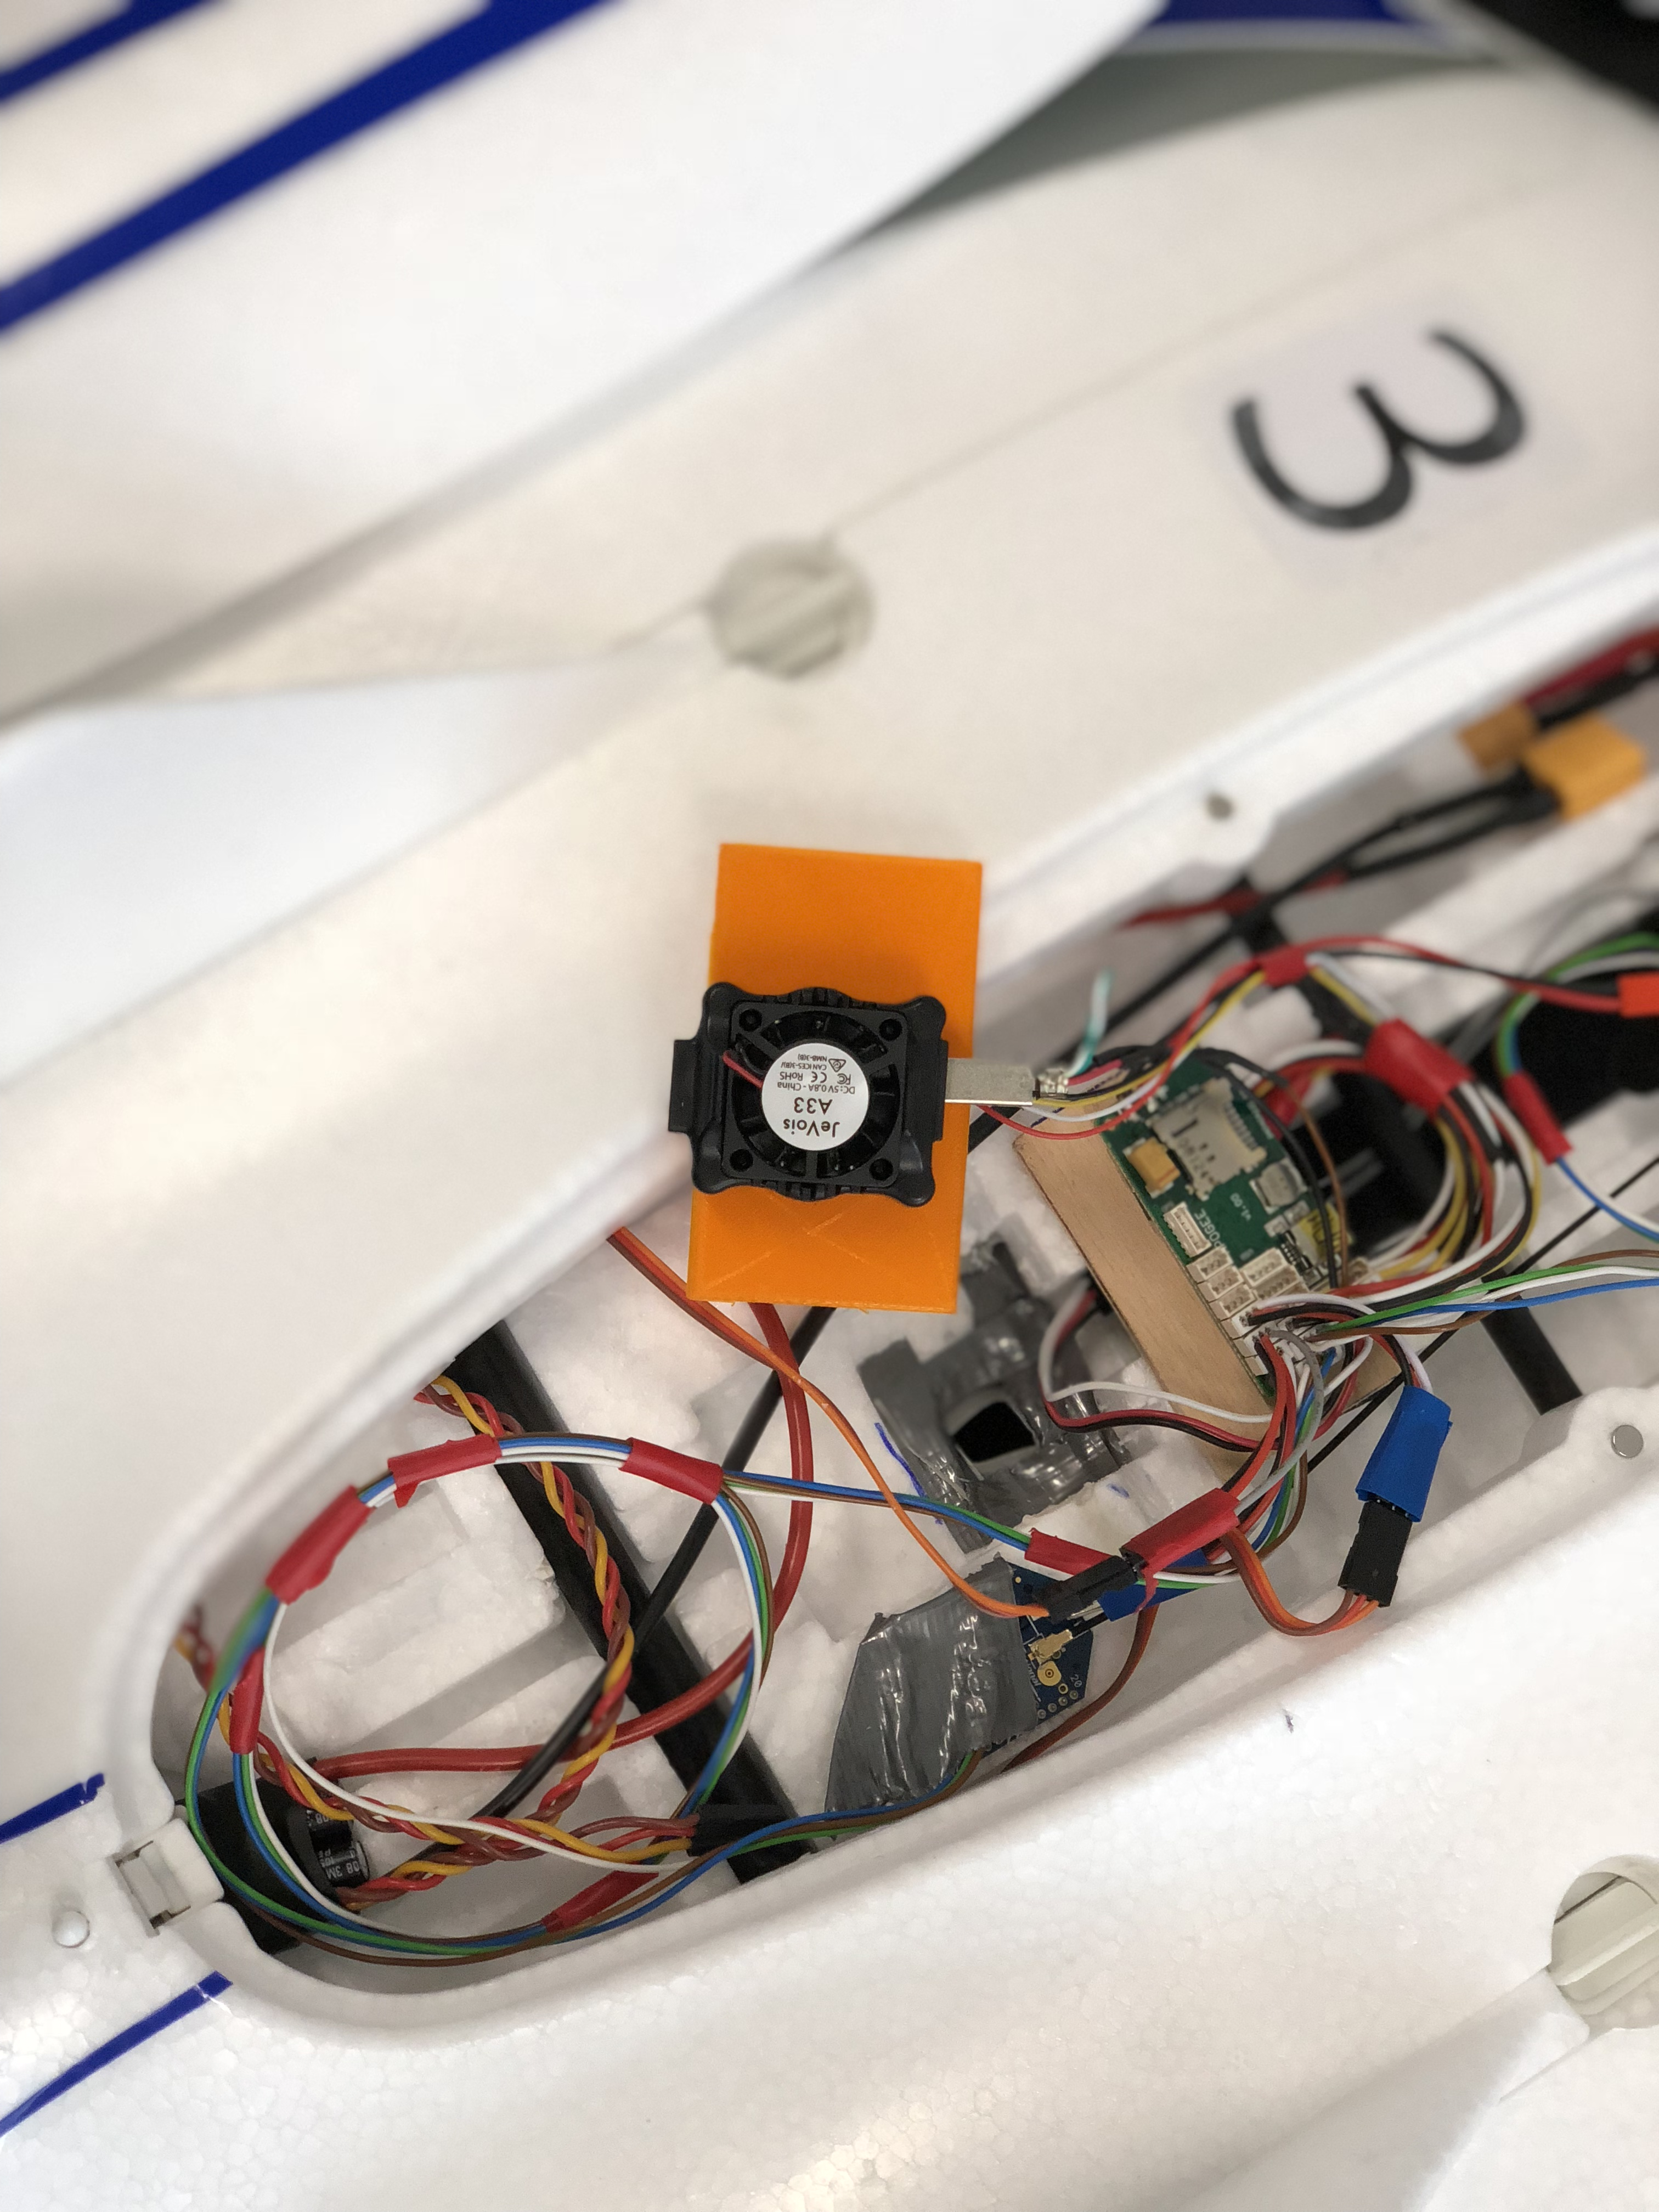
\includegraphics[width=10cm,height=10cm,keepaspectratio]{imagenes/jevois.jpg}
\caption{JeVois camera}
\label{fig:jevois}
\end{figure}
